
\begin{frame}
    \frametitle{前情回顾}
    学习量子光学的必要性
    \begin{itemize}
        \Item 经典光学(麦克斯韦方程) \\
        <-> 黑体辐射, 光电效应, 康普顿效应, 原子光谱, 自发发射, 受激发射...
        \Item 半经典光学(量子化粒子+经典光场)  \\
        <-> 延迟选择实验, 量子擦除实验, 相干态, 压缩态, 量子计算, 量子通信, 量子存储...
        \Item 量子光学(量子化粒子+量子化光场)   
    \end{itemize}     
\end{frame}

\begin{frame}
    \frametitle{场与粒子}
    物理学基本认识:
    \begin{itemize}
        \item 场是物质存在的基本形式
        \item 所有的粒子都是场的量子
        \item 场量子与量子力学的粒子并不完全一样,在非相对论近似下两者可拟合在一起
        \item 光量子是光场的量子,无非相对论近似,不是量子力学中的粒子
    \end{itemize} 
\end{frame}

%%%%%%%%%%%%%%%%%%%%%%%%%%%%%%%%%%%%%%%%%%%%%%%%%%%%%%%%%%%%%
\begin{frame} [plain]
    \frametitle{}
    \Background[1] 
    \begin{center}
    {\huge 第2-3讲:量子力学基础}
    \end{center}  
    \addtocounter{framenumber}{-1}   
\end{frame}
%%%%%%%%%%%%%%%%%%%%%%%%%%%%%%%%%%%%%%%%%%%%%%%%%%%%%%%%%5%%%

\section{1.量子态与希尔伯特空间}

\begin{frame} 
    \frametitle{希尔伯特空间}
    量子态用希尔伯特空间的矢量描述\\
    \begin{equation*}
        \begin{split}
            \text{1、定义加法} \quad  &\xi=\psi+\varphi\\
            &\psi+\varphi=\varphi+\psi \qquad (\text{交换律})\\
            &(\psi+\varphi)+\xi=\psi+(\varphi+\xi) \qquad (\text{结合律})\\
            &\psi+\text{O}= \psi \qquad (\text{零元})\\
            &\psi+\varphi= \text{O} \qquad (\text{逆元})\\
        \end{split}  
    \end{equation*}
\end{frame} 

\begin{frame} 
    \begin{equation*}
        \begin{split}
            \text{2、定义数乘} \quad &\varphi=\psi a\\
            &\psi 1= \psi \qquad (\text{1元})\\
            &(\psi a)b=\psi (ab) \qquad (\text{结合律})\\
            &\psi(a+b)= \psi a+ \psi b \qquad (\text{第一分配律})\\
            &(\psi+\varphi) a= \psi a +\varphi a \qquad (\text{第二分配律})\\
        \end{split}  
    \end{equation*}
\end{frame} 

\begin{frame} 
    \begin{equation*}
        \begin{split}
            \text{3、定义内积} \quad &c=(\psi, \varphi)\\
            &(\psi, \varphi)= (\varphi,\psi)^* \\
            &(\psi, \varphi+\xi)= (\psi, \varphi) + (\psi, \xi)\qquad (\text{分配律})\\
            &(\psi, \varphi a)= (\psi, \varphi )a \\
            &(\psi a, \varphi )= a^* (\psi, \varphi ) \\
            &(\psi,\psi)= c\ge 0\\
        \end{split}  
    \end{equation*}
\end{frame}

\begin{frame} 
    \例 [0. 有定义在$C^n$空间的列矩阵,求内积]
    { \[\psi=
        \begin{pmatrix}
                a_1\\
                a_2\\
                a_3
        \end{pmatrix}, \qquad 
        \varphi =\begin{pmatrix}
            b_1\\
            b_2\\
            b_3
    \end{pmatrix}
     \] 
    }
    \解 ~ \[(\psi, \varphi) = \begin{pmatrix}
        a_1 ^* &
        a_2 ^* &
        a_3 ^*
    \end{pmatrix}
        \begin{pmatrix}
        b_1\\
        b_2\\
        b_3
    \end{pmatrix}
    =a_1 ^* b_1 +a_2 ^* b_2 +a_3 ^* b_3
    =c 
    \]
    ~ \[(\varphi,\psi) = \begin{pmatrix}
        b_1 ^* &
        b_2 ^* &
        b_3 ^*
    \end{pmatrix}
        \begin{pmatrix}
        a_1\\
        a_2\\
        a_3
    \end{pmatrix}
    =b_1 ^* a_1 +b_2 ^* a_2 +b_3 ^* a_3
    =c^* 
    \]
\end{frame} 

\begin{frame} 
    \例 [1. 求定义在x空间的函数的内积]{}

    \解 ~ \[(\psi, \varphi)=\int_a ^b \psi^*(x)  \varphi(x) dx =c\]
    \[(\varphi,\psi)=\int_a ^b \varphi^*(x)\psi(x) dx = (\int_a ^b \varphi(x)\psi^*(x) dx) ^* =c^*\]
\end{frame} 

\begin{frame}
    4、定义空间\\
   \begin{itemize}
       \Item 矢量空间:满足加法和数乘两种运算的集合
       \Item 内积空间:满足加法、数乘和内积三种运算的集合
       \Item 希尔伯特空间:  完全的内积空间\\
       ~~ \\
       *完全性:对给定任意小的实数$\varepsilon$,总有数N存在,当m, n>N时,有\\
       $$ (\psi_m -\psi_n, \psi_m -\psi_n )< \varepsilon $$
   \end{itemize} 
   \Tips ~ 量子体系的状态用希尔伯特空间的矢量描述
\end{frame} 

\begin{frame}
    5、几个概念\\
   \begin{itemize}
       \Item 模(方):$|\psi|^2= (\psi, \psi)=c$
       \Item 归一化: $|\psi|^2= (\psi, \psi)=c=1$
       \Item 正交性(线性无关):  $(\psi, \varphi)=0 $ \\
       \Item 完全集: 有一组线性无关集,如果空间的任意矢量都可以在其上展开,则称它为一个完全集,记为$\{\phi_i\}$
       \[\psi=\sum_i a_i \phi_i= \sum_i (\phi_i,\psi) \phi_i\]
       \Item 维度:最小完全集所包含矢量的数目相同,称这个数目为空间的维度
       \Item 正交归一完全集:对于一个n维的完全集,有:\[(\phi_i,\phi_j)=\delta_{ij}, \qquad i,j=1,2,3,\cdots, n \]
       \Item 基与基矢:称一个正交归一完全集为空间的一个基,它所含的矢量称不计算基矢
   \end{itemize} 
\end{frame} 

\begin{frame}
 \Tips~ 同一空间可以有不同的基,\\
 $C^2$空间的一个基:
 \[ \rs{0}\equiv\begin{bmatrix}
     1 \\
     0
 \end{bmatrix}; \qquad \rs{1}\equiv\begin{bmatrix}
    0 \\
    1
\end{bmatrix} \]

$C^2$空间的另一个基:
\[ \rs{+}\equiv\frac{1}{\sqrt{2}}\begin{bmatrix}
    1 \\
    1
\end{bmatrix}=\Pstate; \qquad \rs{-}\equiv\frac{1}{\sqrt{2}}\begin{bmatrix}
   1 \\
   -1
\end{bmatrix}=\Mstate \]
它们可以相互转换.
\end{frame} 

\begin{frame} 
    例: 若$\rs{0}, \rs{1}$描述垂直和水平偏振, 则 $\rs{+}, \rs{-}$ 描述正负45度偏振. 
    \begin{center}
        \begin{overpic} [width=0.7\textwidth]{figs/26.png}
            %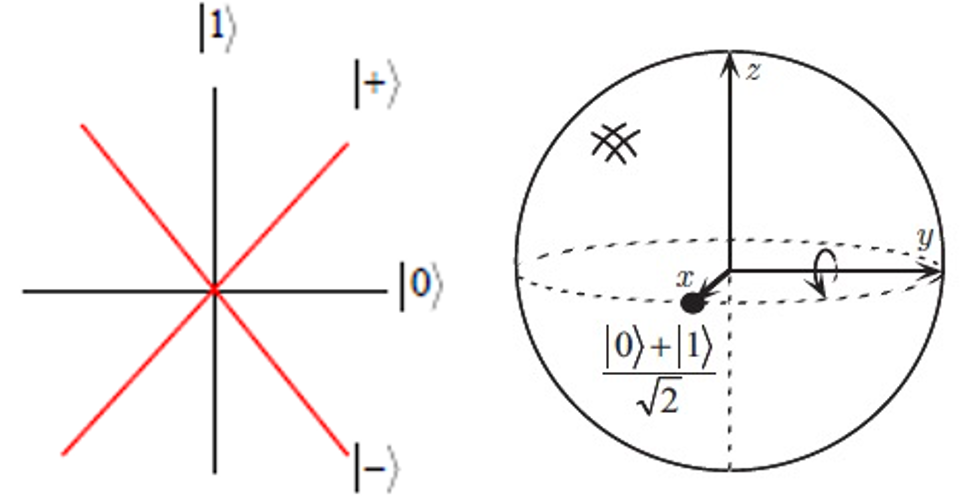
\includegraphics[width=0.7\textwidth]{figs/26.png}
            \put(72,48){\small\bfseries \color{red}{$|1\rangle$}}
            \put(72,-1){\small\bfseries \color{red}{$|0\rangle$}}
        \end{overpic}   
    \end{center} 
    若$\rs{0}, \rs{1}$描述在Z方向自旋投影, 则 $\rs{+}, \rs{-}$ 描述在X方向的自旋投影. 
\end{frame}

\begin{frame}{}
    6、左矢与右矢\\
    考察内积: $(\psi,\psi)=\int\psi^*\psi d\tau$ \\
    同一波函数放在左边还是右边,意义有所不同: \\
    右边是线性的:  $(\psi,a\psi)=(\psi,\psi)a $ \\
    左边是反线性的:   $(a\psi,\psi)=a^* (\psi,\psi)$  \\
    为清楚描述线性反线性特点,定义左矢和右矢, 写狄拉克记号
    $$\langle \psi |, \qquad |\psi \rangle $$ 
    数乘性质: $$\langle a\psi | = \langle \psi |a^* $$
    $$ |a\psi \rangle = a|\psi \rangle$$ 
    内积:\[(\psi,\varphi)\equiv \langle \psi | \varphi \rangle\]
\end{frame}

\begin{frame}{}
    7、外积\\
    考察展开式: \[\psi=\sum_i a_i \phi_i= \sum_i (\phi_i,\psi) \phi_i\]
    \[\rs{\psi}=\sum_i a_i \rs{\phi_i}= \sum_i \lr{\phi_i}{\psi} \rs{\phi_i} =\sum_i \rl{\phi_i}{\phi_i} \rs{\psi}\]
    ~~\\
    令 $p_i= \rl{\phi_i}{\phi_i} $, 称为外积\\ {\vspace*{1em}}
    完备性:
    \[\sum_i p_i= \sum_i \rl{\phi_i}{\phi_i}=1 \]
\end{frame}

\begin{frame}{}
        \例 [2. 有定义在$C^n$空间的列矩阵,求内积和外积]
        { \[\rs{\psi}=
            \begin{pmatrix}
                    a_1\\
                    a_2\\
                    a_3
            \end{pmatrix}, \qquad 
            \rs{\varphi} =\begin{pmatrix}
                b_1\\
                b_2\\
                b_3
        \end{pmatrix}
         \] 
        }
        \解 ~ \[\lr{\psi}{\varphi} = \begin{pmatrix}
            a_1 ^* &
            a_2 ^* &
            a_3 ^*
        \end{pmatrix}
            \begin{pmatrix}
            b_1\\
            b_2\\
            b_3
        \end{pmatrix}
        =a_1 ^* b_1 +a_2 ^* b_2 +a_3 ^* b_3
        =c 
        \]
        ~ \[\rl{\psi}{\varphi} = \begin{pmatrix}
            a_1  \\
            a_2  \\
            a_3 
        \end{pmatrix}
            \begin{pmatrix}
            b_1 ^* &
            b_2 ^* &
            b_3 ^*
        \end{pmatrix}
        =  \begin{pmatrix}
            a_1b_1 ^* & a_1b_2 ^* & a_1b_3 ^* \\
            a_2b_1 ^* & a_2b_2 ^* & a_2b_3 ^* \\
            a_3b_1 ^* & a_3b_2 ^* & a_3b_3 ^* 
        \end{pmatrix}
        \]
\end{frame}

\begin{frame} 
\frametitle{}
 \例 [3. 求如下波函数的外积]{
 \[\rs{\psi}= a_1 \rs{1} + a_2 \rs{2}, \quad \rs{\varphi}= b_1 \rs{1} + b_2 \rs{2} \]}
 \解 ~(1) 代数形式 
   \[ \begin{aligned}
    \rl{\psi}{\varphi} &= (a_1 \rs{1} + a_2 \rs{2}) (\ls{1}b_1 ^*  + \ls{2} b_2 ^* )\\
      &= a_1 b_1 ^* \rl{1}{1} + a_2 b_2 ^* \rl{2}{2} + a_1 b_2 ^* \rl{1}{2} + a_2 b_1 ^* \rl{2}{1} \\
   \end{aligned}\]   
* 后两项为耦合项\\ 
(2) 矩阵形式
~ \[\rl{\psi}{\varphi} = \begin{pmatrix}
    a_1  \\
    a_2  
\end{pmatrix}
    \begin{pmatrix}
    b_1 ^* &
    b_2 ^* &
\end{pmatrix}
=  \begin{pmatrix}
    a_1b_1 ^* & a_1b_2 ^*  \\
    a_2b_1 ^* & a_2b_2 ^*  
\end{pmatrix}
\]
* 非对称元为耦合项
\end{frame}

\section{2.物理量与算符}

\begin{frame}
    \frametitle{算符}
    物理量用希尔伯特空间的线性厄密算符描述\\
    1. 定义:
    \begin{itemize}
        \Item 算符:描述态矢量之间的映射关系,算符作用于一个态映射到另一态。
        \[F \rs{\Psi}=\rs{\psi}\]
        \Item 算符相等: 对任意态$\rs{\psi}$, 恒有下式, 则 $A= B$ \[ A\rs{\psi}=B\rs{\psi}\]
        \Item 单位算符: \[I\Psi=\Psi \]
        \Item 算符的和:  
        $$ (A+B)\Psi=A\Psi+B\Psi $$   
    \end{itemize}
\end{frame} 

\begin{frame}
 \frametitle{}
 \begin{itemize}
    \Item 算符的积 
    $$ (AB)\Psi=A(B\Psi) $$
    * 不存在交换律,即 $AB=BA$ 或 $AB\ne BA$ 皆有可能 \\
    定义对易子来描述 \\
    $$ [A,B]=AB-BA$$
    若[A,B]=0,称两算符对易(可交换),否则不对易(不可交换)
    \Item 逆算符  
    \[F^{-1}\rs{\psi}=\rs{\Psi} \] 
    \Item 线性算符 \[F (a\rs{\Psi} +b\rs{\psi}) = aF \rs{\Psi} +bF\rs{\psi}\]
\end{itemize}
\end{frame}

\begin{frame}
    \frametitle{}
    \begin{itemize}
        \Item 伴算符   \[\ls{\psi}=\ls{\Psi}F^{\dagger} \]
        \[F^{\dagger} = (F^* _{nm})^T \]
        \Item 自伴(厄密)算符  \[F = F^{\dagger} \] 
        性质(1): $\lr{\Psi F}{\psi}=\lr{\Psi }{F \psi}=\lcr{\Psi }{F} {\psi}$ \\
        性质(2): $\lcr{\Psi }{F} {\psi}=\lcr{\psi }{F} {\Psi}^*$ \\ \vspace{0.6em}
        \Item 幺正(酉)算符    \[F^{-1} = F^{\dagger} \] 性质: $FF^{\dagger}=F^{\dagger}F=I$, 通常写成 $UU^{\dagger}=U^{\dagger}U=I$ \\ \vspace{1.0em}
    \end{itemize}        
\end{frame}

\begin{frame}
    \frametitle{}
    \Tips 幺正(酉)变换实现空间变换: 把一个空间所有矢量都用同一幺正算符作用,得到的另一个新的空间,
    \[U\rs{\Psi} =\rs{\Psi'}\]
    {\Bullet}~新旧空间算符之间的关系: \\
        旧空间的算符: \[F \rs{\Psi}=\rs{\varphi}\]
        新空间的算符: \[F' \rs{\Psi'}=\rs{\varphi'}\]
        关系:
        \[F' U\rs{\Psi}=U\rs{\varphi}\]
        \[F' U\rs{\Psi}=UF \rs{\Psi}\]
        \[U^{\dagger}F' U\rs{\Psi}=U^{\dagger}UF \rs{\Psi}\]
        \[U^{\dagger}F' U=F \]
\end{frame}

\begin{frame}
    \frametitle{}
    \begin{itemize}
    \Item 投影算符: 基矢的外积是一种投影算符,
    \end{itemize}
    对于展开式: 
    \[\rs{\psi}=\sum_i a_i \rs{\phi_i}=\sum_i \rs{\phi_i} \lr{\phi_i}{\psi}=\sum_i p_i \rs{\psi} =\sum_i \rs{\psi_i}\]
    有:\[p_i \rs{\psi} =\rs{\psi_i}\]
    即,外积$\rl{\phi_i}{\phi_i}$作用于$\rs{\psi}$,得到第$i$个基矢态上的投影分量!\\
\end{frame}

\begin{frame}    
    \begin{itemize}
        \Item 测量算子: 常称投影算符为测量算子. 对于$C^2$空间, 定义为:
        \end{itemize}
    \[M_0=\rl{0}{0}, \qquad M_1=\rl{1}{1} \]
    具有$2\times 2$的矩阵形式,
    可以证明:\\
    {\bullet} 测量算子是自伴(厄密)算符 :\[M_m = M_m ^{\dagger} \]
    {\bullet} 平方不变性 :\[M_m ^2 = M_m \]
    {\bullet} 完备性 :\[M_0 + M_1 = M_0 ^2 + M_1 ^2 = M_0 M_0 ^\dagger + M_1 M_0 ^\dagger=I\]
\end{frame}

\begin{frame} 
    \frametitle{}
    {\bullet} 测量后的态函数 
    \[\begin{aligned}
        M_0\rs{\Psi} 
        &= \rl{0}{0}(a_0\rs{0}+a_1\rs{1})  \\ 
        &= \rl{0}{0}a_0\rs{0}  \\ 
        &= a_0\rs{0}  \\ 
        &= \frac{a_0}{|a_0|}\rs{0}  \qquad \text{(归一化)} \\ 
    \end{aligned}\]    
    {\bullet} 测得的概率(密度) 
    \[\begin{aligned}
        \lcr{\Psi}{M_0 ^\dagger M_0}{\Psi} 
        &= \lcr{0 }{a_0 ^* a_0} {0} \\ 
        &= \lr{0 }{0}a_0 ^* a_0 \\ 
        &= |a_0|^2 = p(0) 
    \end{aligned}\] 
    重写测量后的状态 \[  M_m\rs{\Psi} = \frac{a_m\rs{m}}{\sqrt{\lcr{\Psi}{M_m ^\dagger M_m}{\Psi}}} = \frac{M_m\rs{\Psi}}{\sqrt{\lcr{\Psi}{M_m ^\dagger M_m}{\Psi}}}\]
\end{frame}

\begin{frame}
    \frametitle{}
    ~\\
    2. 算符的代数形式 \\ {\vspace*{0.3em}}
 {\Bullet}位置算符和动量算符
\例[4.已知粒子的位置波函数$\psi(x,t)$,求动量的期望值]{}   
\解~ 由概率诠释,位置期望值为
\begin{equation*}
    \bar{x}=\int x|\psi(x, t)|^{2} d x=\int \psi^{*}(x, t) x \psi(x, t) d x
\end{equation*}
对于动量波函数 $c(p,t)$, 动量期望值为
\begin{equation*}
    \bar{p_x}=\int p_x|c(p_x, t)|^{2} d p_x=\int c^{*}(p_x, t) p c(p_x, t) d p_x
\end{equation*}
很明显,有
\begin{equation*}
    \bar{p_x}\neq\int p_x|\psi(x, t)|^{2} d p_x
\end{equation*}
\end{frame} 

\begin{frame}
变换求解
\begin{equation*}
    \begin{split}
        \bar{p}&=\int c^{*}(p) p c(p) d p \\  
        &=\int (\frac{1}{\sqrt{2 \pi \hbar}} \int \psi^{*}(x) e^{\frac{i}{\hbar} p\cdot x} d x) p c\left(p\right) d p \\
        &=\frac{1}{\sqrt{2 \pi \hbar}} \int \int \psi^{*}(x) (e^{\frac{i}{\hbar} p\cdot x}  p) c\left(p\right) d xd p \\
        &=\frac{1}{\sqrt{2 \pi \hbar}} \int \int \psi^{*}(x) \Myitem{t1}{red}{(-i\hbar\frac{d}{d x} e^{\frac{i}{\hbar} p\cdot x})} c(p) d xd p \\
        &=\int \psi^{*}(x) (-i\hbar\frac{d}{d x}) (\frac{1}{\sqrt{2 \pi \hbar}} \int e^{\frac{i}{\hbar} p\cdot x} c(p) d p)  d x\\
        &=\int \psi^{*}(x) (-i\hbar\frac{d}{d x}) \psi(x)  d x\\
     \end{split}
\end{equation*}  
\end{frame} 

\begin{frame}
定义如下计算符号:
$$ \boxed{\hat{p}_x= -i\hbar\frac{d}{d x}} $$ 
上式变为:         
$$\boxed{\bar{p}_x=\int \psi^{*}(x) \hat{p}_x \psi(x) d x} $$
称$ \hat{p}_x= -i\hbar\dfrac{d}{d x} $ 为位置表象里的动量算符表示($p_x$分量)\\
同理,称 $\hat{x}= x $ 为位置表象里的位置算符表示($x$分量)\\ \vspace{0.3em}
存在量子力学基本对易关系 \[ [\hat{x},\hat{p}_x]=i\hbar\] 
\end{frame}

\begin{frame} 
    \frametitle{}
    {\Bullet} 任意力学量的算符
    \begin{tcolorbox1}{命题:}
    已知位置、动量的算符表示如下,
    \begin{itemize}
        \Item  位置算符(三维): $ \hat{\vec{r}} =\vec{r} $
        \Item  动量算符(三维): $ \hat{\vec{p}} =-i\hbar(\dfrac{d}{d x}, \dfrac{d}{d y} , \dfrac{d}{d z})=-i\hbar \nabla $
    \end{itemize}
    求任意其他力学量的算符
    \end{tcolorbox1}
    \alert{Bohm规则(1):} 经典物理学的力学量F,若是位置与动量的函数
    \[F(\vec{r},\vec{p})\]
    则其量子力学算符为:
    \[\hat{F}=F(\hat{\vec{r}},\hat{\vec{p}})\]
\end{frame} 

\begin{frame}
    \frametitle{}     
{\Bullet}正则位置和正则动量
  \[ \frac{\mathrm{d }q}{\mathrm{d }t} = \frac{\partial H(q,p) }{\partial p}, \quad \frac{\mathrm{d }p}{\mathrm{d }t} = -\frac{ \partial H(q,p) }{\partial q} \]
  正则位置和正则动量算符的对易关系
  \[ [\hat{q},\hat{p}]=i\hbar\]
  \alert{Bohm规则(2):} 经典物理学存在力学量F,是正则位置与动量的函数
  \[F(q,p)\]
  则其量子力学算符为:
  \[\hat{F}=F(\hat{q},\hat{p})\]
  量子涨落关系(不确定性原理) \[\overline{(\Delta \hat{q})^2} \cdot \overline{(\Delta \hat{p})^2} \geq  \frac{1}{4} \hbar ^2 \]
\end{frame} 

\begin{frame}
    \frametitle{}
    3. 算符的矩阵形式
    \[\begin{aligned}
        \rs{\psi}&=F \rs{\Psi} \\
        \lr{i}{\psi}&= \lcr{i}{F}{\Psi} \\
        \lr{i}{\psi}&= \sum_j\lcr{i}{F}{j}\lr{j}{\Psi} \\
        \lr{i}{\psi}&= \sum_j F_{ij}\lr{j}{\Psi}
    \end{aligned}\]  
    算符矩阵元公式:\[ F_{ij}=\lcr{i}{F}{j}\]
    伴算符的矩阵等于原算符的厄密共轭:\[ F^{\dagger}=(F_{ij} ^*)^T\]
\end{frame}

\begin{frame}
    \frametitle{}
    4. 算符的本征方程
    \begin{itemize}
        \Item 定义式: \[F \rs{n}=f_n\rs{n}\]
        \Item 相关定理:
        \begin{itemize}
            \IItem 厄密算符的本征值是实数
            \IItem 厄密算符的所有本征矢构成正交归一完全集
            \IItem 当且仅当两厄密算符互相对易时才俱有共同的本征矢完全集
            \IItem 完全确定一个量子态所需要的彼此对易的一组力学量算符的最小集称为力学量完全集,所含力学量数目与体系的自由度数目相同
            \end{itemize}
    \end{itemize}
\end{frame}

\section{3.狄拉克记号量子力学}

\begin{frame} 
    \frametitle{狄拉克记号的量子力学}  
    量子态(无表象): $\hspace{1em}|\Psi \rangle, \quad$ 位置表象:$\hspace{1em} \langle x |\Psi \rangle , \quad$ 动量表象:$\hspace{1em} \langle p_x |\Psi \rangle$ \\ \vspace{0.1em}
    算符: $F, \quad$ 位置表象:$\hspace{1em} F(x, -i\hbar \frac{\partial }{\partial x}) , \quad$ 动量表象:$\hspace{1em} F(i\hbar \frac{\partial }{\partial p_x}, p_x) $ \\ \vspace{0.1em}
    展开式: $\hspace{1em}|\Psi \rangle =\sum\limits_{n=1} ^n a_n |n \rangle$ \\
    内积:   $\hspace{2em}\langle \varphi | \Psi \rangle = (\varphi, \Psi)= \int \varphi^*\Psi d\tau $ \\  \vspace{0.1em}
    归一化: $\hspace{1em}\langle \Psi | \Psi \rangle = (\Psi, \Psi)= \int \Psi^*\Psi d\tau = 1 $ \\ \vspace{0.1em}
    正交归一: $\langle n | m \rangle = \delta_{nm} $ \\ \vspace{0.1em}
    $ \hspace{5em} \langle \lambda | \lambda' \rangle = \delta(\lambda-\lambda') $\\ \vspace{0.2em}
    展开系数: $ a_n= \langle n | \Psi \rangle$ \\ \vspace{0.2em}
    展开系数: $ a_n ^*= \langle \Psi | n \rangle$ \\ \vspace{0.2em}
\end{frame} 
 
\begin{frame} 
    平均值:  $\hspace{1em}\bar{F} = \langle \Psi |F | \Psi \rangle$ \\ \vspace{0.2em}
    矩阵元:  $\hspace{1em}F_{nm} = \langle n |F | m \rangle$ \\ \vspace{0.2em}
    幺正变换:$S_{m\alpha} =\langle m| \alpha \rangle $ \\ \vspace{0.2em}
    投影算符:$p_i = |i\rangle\langle i |, \quad \text{封闭性:} \sum_i |i\rangle\langle i |=1 $ \\ \vspace{0.2em}
    本征方程:$F|n\rangle =f_n |n\rangle$ \\ \vspace{0.2em}
    薛定谔方程:$$ i\hbar \frac{\partial }{\partial t} |\Psi(t)\rangle = H|\Psi(t)\rangle $$ 
    算符运动方程:$$ \frac{d\bar{A}(t)}{dt}=\overline{(\frac{\partial A(t) }{\partial t})}  +\frac{1}{i\hbar} \overline{[A(t),H(t)]}$$
\end{frame} 

\begin{frame} 
    \例 [求薛定谔方程在各表象中的形式]{} 
    $$ \begin{aligned}
    i \hbar \frac{\partial}{\partial t} |\Psi(t) \rangle &= H |\Psi(t) \rangle  , \quad \text{无表象}\\
    i \hbar \frac{\partial}{\partial t} \langle x|\Psi(t) \rangle &= H (x, \hat{p}_x) \langle x|\Psi(t) \rangle  , \quad \text{位置表象}\\
    i \hbar \frac{\partial}{\partial t} \langle x|\Psi(t) \rangle &= [- \frac{\hbar^2}{2\mu} \frac{\partial ^2 }{\partial x^2} + U(x)] \langle x|\Psi(t) \rangle  , \quad \text{位置表象}\\
    i \hbar \frac{\partial}{\partial t} \langle p_x|\Psi(t) \rangle &= H (\hat{x}, p_x) \langle p_x|\Psi(t) \rangle  , \quad \text{动量表象}\\
    i \hbar \frac{\partial}{\partial t} \langle p_x|\Psi(t) \rangle &=  [ \frac{p^2 _x}{2\mu} + U(i \hbar \frac{\partial }{\partial p_x}) ] \langle p_x|\Psi(t) \rangle  , \quad \text{动量表象}\\
    i \hbar \frac{\partial}{\partial t} \langle n|\Psi(t) \rangle &=  \langle n|H|m \rangle \langle n |\Psi(t) \rangle  , \quad \text{Q表象}\\
    \end{aligned}
    $$
\end{frame} 

\begin{frame} 
 \frametitle{密度算符}
    
    设系统以$P_i$的概率出现$\rs{\psi_i}$ 态上, 求物理量F的平均值:\\ 
    (1) 物理量F在$\rs{\psi_i}$的均值
    \[\overline{F_i}=\ls{\psi_i}F \rs{\psi_i}
    \]
    (2) 测得$\overline{F_i}$的概率为$P_i$,所以均值为
    \[\overline{F}= \sum_i P_i \overline{F_i}\]
\end{frame}

\begin{frame} 
 \frametitle{} ~\\
      \例 [5. 若物体处于纯态, 即其状态能用一个态矢量$\rs{\psi}$描述, 求物理$F$的平均值] {
      \[ \begin{aligned}
          \overline{F} &= \lcr{\psi}{F}{\psi} \\
          &= \sum_n \lcr{\psi}{F}{n}\lr{n}{\psi}   \\
          &= \sum_n \lr{n}{\psi} \lcr{\psi}{F}{n} \\ 
          &=  \sum_n \lcr{n}{\rho F}{n} \\
          &= Tr (\rho F)
      \end{aligned}\] }
    式中定义了纯态$\rs{\psi}$的密度算符:
    \[\rho = \rl{\psi}{\psi}  \]
\end{frame}

\begin{frame} 
 \frametitle{}
 ~\\
 \例 [5'. 若物体处于混态,则要用一系列场矢量\{$\rs{\psi_i}$\}描述. 设测量其处于$\rs{\psi_i}$的概率为$P_i$, 求物理$F$的平均值] { 
      \[ \begin{aligned}
        \overline{F} &= \sum_i P_i \overline{F_i}\\
        &= \sum_i P_i \ls{\psi_i}F \rs{\psi_i} \\ 
        &= \sum_i P_i \sum_n \lcr{\psi_i}{F}{n}\lr{n}{\psi_i} \\
        &= \sum_n\ls{n} (\sum_i P_i \rl{\psi_i}{\psi_i} )F \rs{n} \\ 
        &= \sum_n\ls{n} \rho F\rs{n} = Tr (\rho F)
      \end{aligned}\] } 
      式中定义了混态的密度算符:
      $\rho = \sum_i P_i\rl{\psi_i}{\psi_i} $ 
\end{frame}

\begin{frame} 
 \frametitle{密度算符的性质}
 用密度算符求平均值, 纯态与混态的公式相同
 \[\overline{F} = Tr (\rho F) \]
 因此,上述公式应用广泛  \\ {\vspace*{2.3em}}

 有必要了解密度算符的性质
 \end{frame}
 
 \begin{frame} 
     \frametitle{}
      (1) 厄密性 $\rho ^{\dagger} = \rho$  \\ 
    \证~ 
    \[ \begin{aligned}
        \rho ^{\dagger} &= (\sum_i P_i\rl{\psi_i}{\psi_i} )^{\dagger} \\
        &= \sum_i P_i(\rl{\psi_i}{\psi_i} )^{\dagger} \\
        &= \sum_i P_i\rl{\psi_i}{\psi_i}  \\
        &= \rho
    \end{aligned}\] 
\end{frame}

\begin{frame} 
 \frametitle{}
      (2) 归一性 Tr($\rho$)=1 \\ 
      \证~
      \[ \begin{aligned}
        Tr(\rho) &= \sum_n \sum_i \lcr{n}{P_i\rl{\psi_i}{\psi_i}}{n} \\
        &= \sum_n \sum_i P_i \lr{n}{\psi_i} \lr{\psi_i}{n}  \\
        &= \sum_n \sum_i P_i a_n^* a_n \\ 
        &= \sum_i P_i \sum_n a_n^* a_n \\ 
        &= \sum_i P_i \\ 
        &=1
      \end{aligned}\] 
      量子概率: $\omega_n= a_n^* a_n$,不可消除.\\ 
      经典概率: $P_i$,没有掌握体系所有信息造成的, 可以消除.
\end{frame}

\begin{frame} 
 \frametitle{}
      (3)  $Tr(\rho^2)\leq 1$  \\ 
      \证~
      \[ \begin{aligned}
        \rho & = \sum_i P_i\rl{\psi_i}{\psi_i} \\ 
        \rho^2 & = \sum_i\sum_j P_iP_j\rl{\psi_i}{\psi_i} \rl{\psi_j}{\psi_j} \\ 
        &= \sum_i\sum_j P_iP_j\rl{\psi_i}{\psi_j} \delta_{ij} \\ 
        &= \sum_i P_iP_i\rl{\psi_i}{\psi_i}  \\
        &=\sum_i P^2_i \rl{\psi_i}{\psi_i} 
    \end{aligned}\] 
    \end{frame}
    
\begin{frame} 
          \frametitle{}  
    \[ \begin{aligned}
        Tr(\rho^2) &= \sum_n \sum_i \lcr{n}{P^2_i\rl{\psi_i}{\psi_i}}{n} \\
        &= \sum_n \sum_i P^2_i\lr{n}{\psi_i}\lr{\psi_i}{n}  \\
        &= \sum_n \sum_i P^2_i a_n^* a_n \\ 
        &= \sum_i P^2_i \sum_n a_n^* a_n \\ 
        &= \sum_i P^2_i \\ 
        &\leq \sum_i P_i \\ 
        &=1
      \end{aligned}\]
    纯态: $Tr(\rho^2) =1$, 混态: $Tr(\rho^2) < 1$. 
\end{frame}

\begin{frame} 
    \frametitle{}
       (4)  $\left\langle \rho \right\rangle   \geq 0 $ \\ 
       \证~
    \[ \begin{aligned}
        \rho & = \sum_i P_i\rl{\psi_i}{\psi_i} \\ 
        \left\langle \rho \right\rangle &= 
        \lcr{n}{\sum_i P_i\rl{\psi_i}{\psi_i}}{n} \\ 
        &= \sum_i P_i \lr{n}{\psi_i}\lr{\psi_i}{n}  \\
        &= \sum_i P_i \left|\lr{n}{\psi_i} \right|^2 \\
        & \geq 0
      \end{aligned}\]   
   \end{frame}

\begin{frame} 
 \frametitle{}
      (5) 对于纯态, 有: $\rho^2 =\rho$ \\ 
      \证~
      \[ \begin{aligned}
        \rho &= \rl{\psi}{\psi}  \\ 
        \rho^2 &= \rl{\psi}{\psi} \rl{\psi}{\psi} \\ 
        &= \rs{\psi}\left\langle \psi | \psi \right\rangle \ls{\psi} \\ 
        &= \rl{\psi}{\psi}  \\ 
        &=  \rho 
      \end{aligned}\]
\end{frame}

\begin{frame} 
\frametitle{}
   (6) 密度算符的运动方程
   \[ \begin{aligned}
    \rho &= \sum_i P_i\rl{\psi_i}{\psi_i}  \\
     i \hbar \frac{\partial \rho}{\partial t} &= \sum_i P_i \left[i \hbar\frac{\partial \rs{\psi_i}}{\partial t}\ls{\psi_i}+ \rs{\psi_i}i \hbar\frac{\partial \ls{\psi_i}}{\partial t}\right] \\ 
     &=  \sum_i P_i \left[ H \rl{\psi_i}{\psi_i} -  \rl{\psi_i}{\psi_i} H \right] \\ 
     &=   \left[ H \sum_i P_i\rl{\psi_i}{\psi_i} - \sum_i P_i \rl{\psi_i}{\psi_i} H \right] \\ 
     &= [H \rho- \rho H] \\ 
     &= [H, \rho] \\ 
     ~\\ 
     i \hbar \frac{\partial \rho}{\partial t} & = [\rho, H]
   \end{aligned}\] 
\end{frame}

\begin{frame} 
\frametitle{}
~\\
    (7) 密度算符的矩阵形式
    \[ \begin{aligned}
       \rs{\Psi} & = a_1\rs{1} + a_2\rs{2} =  \begin{pmatrix}
        a_1  \\
        a_2 
    \end{pmatrix} \\
       \rho & = \rl{\Psi}{\Psi}  = \sum_{i,j=1,2} a_i a_j ^* \rl{i} {j}\\
       \rho & = \begin{pmatrix}
        a_1  \\
        a_2 
    \end{pmatrix} \begin{pmatrix}
        a^* _1  &  a^* _2
    \end{pmatrix}\\
    &= \begin{pmatrix}
        a_1a_1 ^* & a_1a_2 ^*  \\
        a_2a_1 ^* & a_2a_2 ^*  
    \end{pmatrix} \\ 
    &= \begin{pmatrix}
        \rho_{11} & \rho_{12}  \\
        \rho_{21} & \rho_{22}  
    \end{pmatrix} \\ 
    \end{aligned}\]     
\end{frame}

\section{4.多粒子体系与张量空间}

\begin{frame}
    \frametitle{张量空间}
    \begin{tcolorbox4}[张量积]
    对于多粒子体系,比如多光子系统,其所处的空间是子系统希尔伯特空间的张量积。也称直积空间。
    \end{tcolorbox4}
\end{frame}

\begin{frame}
    \frametitle{~1. 张量空间的计算基矢}
    子系统A是n维的,计算基(某厄密算符的本征函数系)为$$\{\rs{\phi_i}\},\quad (i=1,2,3,\cdots,n)$$ 
    子系统B是m维的,计算基为$$\{\rs{\varphi_j}\},\quad (j=1,2,3,\cdots,m)$$ 
    总系统是n张m维的张量空间,计算基为:$$\{\rs{\phi_i}\otimes\rs{\varphi_j}\},\quad (i=1,2,3,\cdots,n;\quad j=1,2,3,\cdots,m)$$ 
    可简写为:$$\{\rs{\phi_i}\otimes\rs{\varphi_j}\}=\{\rs{\phi_i}\rs{\varphi_j}\}=\{\rs{\phi_i\varphi_j}\}=\{\rs{ij}\}$$
\end{frame}

\begin{frame}
    \frametitle{}
    总体系的任意态是计算基矢的叠加态:
    \[ \rs{\Psi} = \sum_{i,j} ^{n,m} a_{ij}\rs{ij}\] \vspace{0.6em}

    \例[7. 写出$C^2$空间的张量空间的计算基]{} 
    \解~基由四个基矢构成$$\{\rs{\phi_i}\otimes\rs{\varphi_j}\}=\{\rs{00},\rs{01},\rs{10},\rs{11}\}$$

矩阵表示是原矩阵的直积,例: 
\[\rs{01} = \rs{0} \otimes \rs{1} =    
\begin{pmatrix}
    1\\
    0
\end{pmatrix}
\otimes
\begin{pmatrix}
    0\\
    1
\end{pmatrix}
=
\begin{pmatrix}
    1 \otimes \begin{pmatrix}
        0\\
        1
    \end{pmatrix}\\
    0 \otimes \begin{pmatrix}
        1\\
        0
    \end{pmatrix}
\end{pmatrix}
=
\begin{pmatrix}
    0\\
    1\\
    0\\
    0
\end{pmatrix}
 \] 
\end{frame}

\begin{frame}
矩阵形式:
    \[
\rs{00} = 
\begin{pmatrix}
    1\\
    0\\
    0\\
    0
\end{pmatrix},\qquad
\rs{01} = 
\begin{pmatrix}
    0\\
    1\\
    0\\
    0
\end{pmatrix},\qquad
\rs{10} = 
\begin{pmatrix}
    0\\
    0\\
    1\\
    0
\end{pmatrix},\qquad
\rs{1} = 
\begin{pmatrix}
    0\\
    0\\
    0\\
    1
\end{pmatrix}
\] 
\end{frame}

\begin{frame}
    \frametitle{}
    双粒子态是四个计算基矢的叠加态:
    \[\rs{\psi} =\alpha_{00}\rs{00}+\alpha_{01}\rs{01}+\alpha_{10}\rs{10}+\alpha_{11}\rs{11}\]
    归一化条件:
    \[ \sum_{ij=0,1} |\alpha_{ij}|^2= 1\]
\end{frame}

\begin{frame}
      \frametitle{ 2. 张量空间的算符}
    子系统A有算符$F_A$, 子系统B有算符$F_B$,总系统可定义它们的张量积
    \[F_{AB}=F_A \otimes F_B\]
    作用于总体系的任意态时,算法为:
    \[F_A \otimes F_B \rs{\Psi} = F_A \otimes F_B \sum_{i,j} a_{ij}\rs{ij}=  \sum_{i,j} a_{ij}F_A \rs{i}\otimes F_B\rs{j}\]   
\end{frame}

\begin{frame}
    \frametitle{~3. 子系统的测量与约化密度矩阵}
    总体系任意(纯)态的密度矩阵
    \[ \rho=\rl{\Psi} {\Psi}= \sum_{i,i',j,j'} a_{i'j'}a_{ij}\rl{i'j'}{ij}\] 
    定义子体系A的约化密度矩阵(把子系统B积分丢!)
    \[ \rho(A)=\sum_{j}\lcr{j}{\rho}{j}=tr_B(\rho)\] 
    测量子体系A的物理量$F_A$的平均值为:
    \[ \bar{F}_A=tr_A(F_A\rho(A))\] 
    
\end{frame}

\section{5.量子力学基本假设}

\begin{frame}
    \frametitle{状态假设}
    \begin{tcolorbox4}[1. 状态假设]
    量子体系的状态用希尔伯特空间的态矢量完全描述。
    \end{tcolorbox4}
    \例[8. 两能级系统用量子比特描述, 它就是2维希尔伯特空间的态矢量]{ 
    \[\rs{\psi} = a_1 \rs{1} + a_2\rs{2}\]
    完全描述两能级系统的所有可能状态}
\end{frame}

\begin{frame}
    \frametitle{演化假设}
    \begin{tcolorbox4}[2. 演化假设]
    一个封闭量子体系的演化用幺正(酉)变换描述。
    \[\rs{\Psi'}=U\rs{\Psi}\]
    状态函数随时间的演化用薛定谔方程描述
    \[ i\hbar \frac{d\rs{\Psi}}{dt}=H \rs{\Psi}\]
    \end{tcolorbox4}
\end{frame}

\begin{frame}
    \例[9. 试证明薛定谔方程与酉变换等价]{}
    \证~ 定义时间演化算符:
    $$ U(t,t_0) |\Psi(t_0)\rangle = |\Psi(t)\rangle  $$
    \alert{分析}:
    (1) 因为 $ U(t_0,t_0) |\Psi(t_0)\rangle = |\Psi(t_0)\rangle  $ \\
    $$ U(t_0,t_0)=I $$
    (2):求 $ U(t,t_0)$
    $$ \begin{aligned}
        i\hbar \frac{\partial }{\partial t} |\Psi(t)\rangle &= H|\Psi(t)\rangle  \\
        i\hbar \frac{\partial }{\partial t}  U(t,t_0) |\Psi(t)\rangle &= H U(t,t_0) |\Psi(t)\rangle  \\
        i\hbar \frac{\partial }{\partial t}  U(t,t_0)  &= H U(t,t_0)  \\
        U(t,t_0)  &= e^{-\frac{i}{\hbar} H(t-t_0)}  \\
    \end{aligned} $$
\end{frame}

\begin{frame}  
    (3):$ U(t,t_0)$是幺正算符
    $$ \begin{aligned}
        U(t,t_0)  &= e^{-\frac{i}{\hbar} H(t-t_0)}  \\
        U^\dagger (t,t_0)  &= e^{\frac{i}{\hbar} H(t-t_0)}  \\
        U^\dagger (t,t_0)U(t,t_0) &= U^\dagger (t,t_0)U(t,t_0) \\
         &=e^{\frac{i}{\hbar} H(t-t_0)-\frac{i}{\hbar} H(t-t_0)} \\
         &=e^0 \\
         &=I
    \end{aligned} $$
    因此,有:
    $$ |\Psi(t)\rangle = |\Psi(t_0)\rangle e^{-\frac{i}{\hbar}H(t-t_0)}   $$
    \Note ~波函数随时间的演化服从的薛定谔方程,只是一种幺正变换。
\end{frame} 

\begin{frame}
 \frametitle{}
    试证明算符的演化方程与薛定谔方程等价 \\ \vspace*{2.3em}
    \[ i\hbar\frac{\mathrm{d A}}{\mathrm{d t}} =  [A, H ] \]
    ~\\ \vspace*{2.3em}
    *参考密度算符运动方程的推导
\end{frame}


\begin{frame}
    \frametitle{量子测量假设}
    \begin{tcolorbox4}[3. 量子测量假设]
    量子测量由一组测量算子$\{ M_m\}$ 描述,测得测量值$m$的概率(密度)为
    \[ p(m)=\lcr{\Psi}{M_m ^\dagger M_m}{\Psi} 
     \]
     测量后的状态 \[\frac{M_m\rs{\Psi}}{\sqrt{\lcr{\Psi}{M_m ^\dagger M_m}{\Psi}}}\]
    \end{tcolorbox4}
\end{frame}

\begin{frame}
    \frametitle{张量积假设}
    \begin{tcolorbox4}[4. 复合系统假设]
    复合系统的状态空间是子系统的状态空间的张量积
    \end{tcolorbox4}
\end{frame}

\begin{frame} 
    \frametitle{}
    ~ \\ 
    {\Bullet}光与两能级原子相互作用体系的两种描述方法 \\ \vspace*{0.6em}
    (1) 光场处于数态 $\rs{n}$,原子处于激发态 $\rs{2}$, 体系的状态为
    \[ \rs{\psi_1}  = \rs{n} \rs{2}\]
    原子放出一个光子后, 回到基态 $\rs{1}$, 光场则处于数态 $\rs{n+1}$, 体系的状态为 
    \[\rs{\psi_2} = \rs{n+1} \rs{1}\]
    体系的所有可能状态用叠加态描述 
    \[\rs{\psi} = a_1 \rs{\psi_1} + a_2\rs{\psi_2}\]
    \end{frame}
    
    \begin{frame} 
        \frametitle{}
        ~ \\ 
        (2) 光场处于数态 $\rs{n}$,原子处于基态 $\rs{1}$, 体系的状态
        \[ \rs{\psi_1}  = \rs{n} \rs{1}\]
        原子吸收一个光子后, 进行激发态 $\rs{2}$, 光场则处于数态 $\rs{n-1}$, 体系的状态为 
        \[\rs{\psi_2} = \rs{n-1} \rs{2}\]
        体系的所有可能状态用叠加态描述 
        \[\rs{\psi} = a_1 \rs{\psi_1} + a_2\rs{\psi_2}\]
    \end{frame}

\begin{frame}
    \frametitle{}
    基于以上4条假设,可以在希尔伯特空间推导整个量子力学(光学)! \\ 

\end{frame}

\section{6.实例}

\begin{frame}
    \frametitle{实例}
    \例 [10. 求解一维谐振子]{}
    \解 (1) 牛顿力学条件下求解: 谐振子在平衡位置附近的振动满足波动方程:
    \begin{equation*}
        u_{tt}=a^2(u_{xx}+ u_{yy}+u_{zz})
    \end{equation*}
    零边界条件求解(一维, $l$为弦长)
    \begin{enumerate}
        \IItem 固有值:$\displaystyle  \lambda~_n=\frac{n^2\pi~^2}{l~^2}$ 
        \IItem 固有解:{$\displaystyle  X~_n(x)=\sin \frac{n\pi~}{l} x=\sin \omega_n x $}
        \IItem 基本解:
        $\displaystyle u_n(x,t) = (a_n\cos\frac{ n\pi at}{l}+ b_n\sin \frac{ n\pi at}{l}) \sin \frac{ n\pi x}{l} $ 
        \IItem 叠加解:
        \[u(x,t) = \sum\limits_{n=1}^{\infty }  (a_n\cos\frac{ n\pi at}{l}+ b_n\sin \frac{ n\pi at}{l}) \sin \frac{ n\pi x}{l}\]
    \end{enumerate}
\end{frame}

\begin{frame}
    \frametitle{}
    \解 (2) 量子力学条件下求解: 先写经典哈密顿量
      \begin{equation*}
          H=T+U = \frac{p^2 }{2m} + \dfrac{1}{2} m \omega ^2 x^2 
      \end{equation*}	
      引入位置与动量算符,$\hat{x}$, $\hat{p}$, 存在对易关系:
      \[ [\hat{x}, \hat{p}] =i\hbar\] 
      得哈密顿量的算符形式
      \begin{equation*}
      \begin{aligned}
          \hat{H} &= \frac{\hat{p}^2 }{2m} + \dfrac{1}{2} m \omega ^2 x^2  \\
                 &= - \frac{\hbar ^2}{2m} \frac{\partial^2 }{\partial x^2 }+ \dfrac{1}{2} m \omega ^2 x^2   
      \end{aligned}
      \end{equation*}	
\end{frame}

\begin{frame}
    \frametitle{}
    把哈密顿量算符代入薛定谔方程, 分离出时间变量后, 得定态薛定谔方程
    \[ \hat{H}\rs{\Psi} =E \rs{\Psi} \]
    求解方程 (复杂, 略), 得: 
    \begin{enumerate}
      \IItem 固有值:$\displaystyle  E_n=(n+\frac{1}{2})\hbar \omega $ 
      \IItem 固有函数:{$\displaystyle  X~_n(x)= H(\alpha x) e^{-(\alpha x)^2 /2 }, \qquad \alpha =\sqrt{\frac{m \omega }{\hbar}} $}
      \IItem 基本解:
      \[ \Psi_n(x,t) = N_n e^{-\frac{i}{\hbar} E_n t } X~_n(x)\]  
      \IItem 叠加解:
      \[ \Psi (x,t) = \sum_n a_n \Psi_n(x,t)\] 
  \end{enumerate}
\end{frame}

\begin{frame}
    \frametitle{}
    \解 (3) 正则量子化求解, 
  \begin{equation*}
      \hat{H} = \frac{\hat{p}^2 }{2m} + \dfrac{1}{2} m \omega ^2 \hat{x}^2   \qquad \text{with} \quad [\hat{x},\hat{p}]=i\hbar 
  \end{equation*}	
  首先验证 $(\hat{x},\hat{p})$ 是一对正则共轭量, 由哈密顿正则方程得: \\ 
  \[ \dot{\hat{x}} = \frac{\partial H }{\partial \hat{p} } =  \frac{{\hat{p}}}{m}; \qquad   \dot{\hat{p}} = - \frac{\partial H }{\partial \hat{x} } = -m \omega ^2 \hat{x} \]
  由这对方程可还原谐振子方程
  \[\frac{\mathrm{d}^2 x}{\mathrm{d} t ^2}  = - \omega^2 x\]
  * 也可以构造别的对称性更好的正则量来求解方程. 比如令: 
  \[ \hat{X} = \sqrt{\frac{m\omega}{\hbar}}\hat{x}, \hat{P} = \sqrt{\frac{1}{m \hbar \omega}} \hat{p} \]
\end{frame}

\begin{frame}
    \frametitle{}
  重写哈密顿量
    \[  \hat{H}= \frac{\hbar \omega }{2} (\hat{X}^2 + \hat{P}^2 ) \qquad \text{with} \quad [\hat{X},\hat{P}]=i \]
  再令:
  \[ \hat{a}= \frac{1 }{\sqrt{2}} (\hat{X} + i\hat{P} ), \qquad \hat{a}^\dagger= \frac{1 }{\sqrt{2}} (\hat{X} - i\hat{P} ) \]
  重写哈密顿量
  \[  \hat{H}= \hbar \omega \left(\hat{a}^\dagger \hat{a} + \frac{1 }{2}\right) \qquad \text{with} \quad [\hat{a},\hat{a}^\dagger]=1 \]
  代入,有:
  \[ \hat{a}= \sqrt{\frac{m\omega}{2\hbar}}\hat{x} + i \sqrt{\frac{1}{2 m \hbar \omega}} \hat{p}, \qquad 
  \hat{a}^\dagger= \sqrt{\frac{m\omega}{2\hbar}}\hat{x} + i \sqrt{\frac{1}{2 m \hbar \omega}} \hat{p}\]
  反向可得:
  \[ \hat{x}= \sqrt{\frac{\hbar}{2m\omega}} (\hat{a}+ \hat{a}^\dagger), \qquad 
  \hat{p}= -i \sqrt{\frac{m \omega \hbar}{2}} (\hat{a}-\hat{a}^\dagger)\]
\end{frame}

\begin{frame}
    \frametitle{}
    很明显,它们是正则的. 现证明对易关系: 
  \[ \begin{aligned}
      [X,P] &=   XP- PX \\ 
      &=  \sqrt{\frac{m\omega}{\hbar}} \sqrt{\frac{1}{m \hbar \omega}}   (xp-px)  {\hspace*{8em}}~~\\
      &=  \sqrt{\frac{m\omega}{\hbar}} \sqrt{\frac{1}{m \hbar \omega}} i \hbar  \\
      &= i
  \end{aligned}\]
   
  \[ \begin{aligned}
       [\hat{a},\hat{a}^\dagger] &=   \hat{a}\hat{a}^\dagger - \hat{a}^\dagger\hat{a} \\ 
       &= \frac{1}{2} (\hat{X} + i\hat{P} )  (\hat{X} - i\hat{P} )  - \frac{1}{2} (\hat{X} - i\hat{P} ) (\hat{X} + i\hat{P} )  \\
       &=  -i (\hat{X}\hat{P}-\hat{P}\hat{X}) \\
       &= -i \times i \\
       &= 1
   \end{aligned}\]
\end{frame}


\begin{frame} 
    \frametitle{}
$ a \not =  a^\dagger $, 说明不具厄密性. 对于能量第n个本征态 \\ 
\[ H  \rs{n} = E_n  \rs{n}, \quad  aH  \rs{n} =E_n a \rs{n}\]
\[
\begin{aligned}
      H a \rs{n} &=\hbar \omega (  a ^\dagger a + \frac{1}{2} )a \rs{n} \\ 
      &= \hbar \omega (   a ^\dagger a a  + \frac{1}{2} a ) \rs{n} \\ 
      &= \hbar \omega (   (-1+a a ^\dagger )a + \frac{1}{2} a ) \rs{n} \\ 
      &= \hbar \omega  (  a a ^\dagger a -  a \frac{1}{2} ) \rs{n} \\ 
      &=  a( a ^\dagger a -  \frac{1}{2} )\hbar \omega \rs{n} 
\end{aligned}
\]
\end{frame}


\begin{frame}
\[ 
\begin{aligned}
  H a \rs{n}  &=  a( \hbar \omega   a ^\dagger a +  \frac{1}{2}\hbar \omega  - \hbar \omega ) \rs{n} \\ 
      &=  (aH - a \hbar \omega ) \rs{n} \\ 
      &=  (E_n -  \hbar \omega ) a\rs{n} \\ 
\end{aligned}
\]
也就是说 $a \rs{n} $ 也是能量本征态, 本征值为 $E_n -  \hbar \omega = E_{n-1} $ 即有一份能量$ \hbar \omega $ 被湮灭, 故称 $a$ 为 湮灭算符 \\ {\vspace*{1.3em}} 

* 存在对易关系:
\[ [H, a ] = - a \hbar \omega \] 
\end{frame}

\begin{frame}
      \frametitle{}
    同理
      \[ 
        \begin{aligned}
          H a^\dagger \rs{n}  
              &=  (a^\dagger H + a^\dagger \hbar \omega ) \rs{n} \\ 
              &=  (E_n +  \hbar \omega ) a^\dagger \rs{n} 
        \end{aligned}
        \]
也就是说 $a^\dagger\rs{n} $ 也是能量本性态, 本征值为 $E_n + \hbar \omega = E_{n+1} $ 即产生一份能量$ \hbar \omega $,
故称 $a^\dagger$ 为产生算符 \\ {\vspace*{1.3em}} 

* 存在对易关系:
\[ [H, a^\dagger ] =  a^\dagger \hbar \omega \] 
\end{frame}


\begin{frame}
本征能量不能被无限湮灭,设最小的为$E_0$, 对应本征态$\rs{0}$, 有:
\[ \boxed{a \rs{0}= 0 }\]
~~\\ 
由 \[H=(a ^\dagger a + \frac{1}{2})\hbar \omega\]  
有: 
\[H-\frac{1}{2}\hbar \omega=\hbar \omega a ^\dagger a \] 
\[ 
\begin{aligned}
(H-\frac{1}{2}\hbar \omega) \rs{0} &= \hbar \omega a ^\dagger a \rs{0} = \hbar \omega a ^\dagger 0 = 0 \\ 
H \rs{0} &= \frac{1}{2}\hbar \omega \rs{0}=E_0 \rs{0} 
\end{aligned}
\] 
即, 谐振子的最低能级为
\[ \boxed{E_0=\dfrac{1}{2}\hbar \omega} \]
\end{frame}


\begin{frame}
称$\rs{0}$ 为真空态. 从真空态出发, 相继使用产生算符,每次产生一份能量 $ \hbar \omega$, 因此谐振子的能量本征值为
\[\boxed{E_n = (n+\frac{1}{2})\hbar \omega, \qquad n=0,1,2, \cdots}  \] 

谐振子被普郞克用来解释黑体辐射场, 即能量本征态$\rs{n}$描述的是该模($\omega$)上占有$n$个激发光子, 每个光子的能量是 $\hbar \omega$ 即 :$\rs{n}$态描述的是含有$n$个光量子的态. 因此,能量本征态$\rs{n}$也称为粒子数态, 也称为$Fock$态. \\

对比 
\[  \hat{H}= \left(\hat{a}^\dagger \hat{a} + \frac{1 }{2}\right) \hbar \omega \]
说明 $a^\dagger a$ 正好描述了 $\rs{n}$态上的粒子数, 令 $\hat{N}=\hat{a}^\dagger \hat{a}$, 称为粒子数算符.
\[ \hat{H}= \left(\hat{N} + \frac{1 }{2}\right) \hbar \omega \] 
\end{frame}

\begin{frame}
  \例 [11. 求粒子数算符$\hat{N}$的本征值和本征函数]{}
  \解~ \[ 
  \begin{aligned}
      \hat{H}\rs{n} & =E_n \rs{n}  \\ 
      \left(\hat{N} + \frac{1 }{2}\right) \hbar \omega \rs{n} & =E_n \rs{n}  \\ 
     \hat{N} \hbar \omega \rs{n} & =(E_n-\frac{1}{2} \hbar \omega) \rs{n}  \\ 
     \hat{N} \hbar \omega \rs{n} & = n \hbar \omega \rs{n}  \\ 
     \hat{N}   \rs{n} & = n  \rs{n}  \\ 
  \end{aligned} 
  \]
  得 $\hat{N}$的本征值为$n$和本征态为 $\rs{n}$ \\ 
  完毕!
\end{frame}

\begin{frame}
    \frametitle{}
    产生湮灭算符分别产生和消灭这个模式的一个光子
    \[ {a \rs{n}= D_n\rs{n-1}}, \qquad a^\dagger \rs{n}= C_n \rs{n+1} \]  
    \[ 
      \begin{aligned}
        a^\dagger a \rs{n} &= a^\dagger D_n\rs{n-1} \\ 
        &= D_n C_{n-1} \rs{n}  \\
        &= n \rs{n} \\ 
        D_n C_{n-1}&=n \qquad \cdots (1)
      \end{aligned}
      \] 
      \[ 
        \begin{aligned}
          D_n &=  \lcr{n-1}{a}{n} \\
          &=  (\lcr{n}{a^\dagger }{n-1})^* \\
          &= C_{n-1} ^*   \qquad \cdots (2)
        \end{aligned}
        \] 
        联立(1)(2), 得 $C_{n-1}=\sqrt{n}= D_n, C_{n}=\sqrt{n+1} $\\  
        \[\boxed{ {a \rs{n}= \sqrt{n}\rs{n-1}}, \qquad a^\dagger \rs{n}= \sqrt{n+1} \rs{n+1}} \]   
\end{frame}

\begin{frame}
    \frametitle{}
    \[ 
  \begin{aligned}
      \rs{n+1} &= \frac{a^\dagger }{\sqrt{n+1}} \rs{n} \\
      \rs{n} &= \frac{a^\dagger }{\sqrt{n}} \rs{n-1} \\
             &= \frac{(a^\dagger)^2 }{\sqrt{n(n-1)}} \rs{n-2} \\
             & \cdots \\
      \rs{n} &= \frac{(a^\dagger)^n }{\sqrt{n!}} \rs{0} \\
  \end{aligned}    
    \]
\end{frame}

\begin{frame}
    \frametitle{}
    \例 [12. 求Fock态在位置表象中的波函数]{}
    \解~ Fock态为$\rs{n}$, 设位置本征态为 $\rs{x}$, 要求 $\psi_n (x)=\lr{x}{n} $  \\
    (1) 求$\psi_0 (x)$
    \[ 
  \begin{aligned}
    0 &= a \rs{0}  \\ 
    &= \ls{x} a \rs{0}  \\ 
    &= \ls{x} \sqrt{\frac{m\omega}{2\hbar}}\hat{x} + i \sqrt{\frac{1}{2 m \hbar \omega}} \hat{p} \rs{0}  \\ 
    &= \ls{x} \sqrt{\frac{m\omega}{2\hbar}} x + \sqrt{\frac{\hbar}{2 m \omega}} \frac{\partial }{\partial x } \rs{0}  \\ 
    &= (\sqrt{\frac{m\omega}{2\hbar}} x + \sqrt{\frac{\hbar}{2 m \omega}} \frac{\partial }{\partial x } )\lr{x}{0}  \\ 
    &= (\sqrt{\frac{m\omega}{2\hbar}} x + \sqrt{\frac{\hbar}{2 m \omega}} \frac{\partial }{\partial x } ) \psi_0 (x) \\ 
  \end{aligned} \] 
  
\end{frame}

\begin{frame}
    \frametitle{}
    解得 \[ 
      \psi_0 (x)=  (\frac{m \omega }{\pi  \hbar})^{\frac{1}{4}}  \exp(- \frac{m \omega }{2 \hbar} x^2) \]
    (2) 求$\psi_1 (x)$
    \[ 
      \begin{aligned}
        \psi_1 (x) &= \lr{x}{1}  \\ 
        &=  \ls{x} \hat{a}^\dagger \rs{0}   \\ 
        &= \ls{x} \sqrt{\frac{m\omega}{2\hbar}}\hat{x} - i \sqrt{\frac{1}{2 m \hbar \omega}} \hat{p} \rs{0}  \\ 
        &= \ls{x} \sqrt{\frac{m\omega}{2\hbar}} x - \sqrt{\frac{\hbar}{2 m \omega}} \frac{\partial }{\partial x } \rs{0}  \\ 
        &= (\sqrt{\frac{m\omega}{2\hbar}} x - \sqrt{\frac{\hbar}{2 m \omega}} \frac{\partial }{\partial x } )\lr{x}{0}  \\ 
        &= \frac{1}{\sqrt{2}} (\xi - \frac{\mathrm{d}}{\mathrm{d}\xi}) \lr{x}{0} 
      \end{aligned} \] 
\end{frame}

\begin{frame}
    \frametitle{}
    (3) 求$\psi_n (x)$
    \[ 
      \begin{aligned}
        \psi_n (x) &= \lr{x}{n}  \\ 
        &=  \frac{1}{\sqrt{n!}}\ls{x} (\hat{a}^\dagger)^n \rs{0}   \\ 
        &=  \frac{1}{\sqrt{n!}}  \frac{1}{\sqrt{2^n}} (\xi - \frac{\mathrm{d} }{\mathrm{d}\xi} )^n (\frac{m \omega }{\pi  \hbar})^{\frac{1}{4}}  e^{- \frac{1 }{2 } \xi^2}    \\ 
        &=  \frac{1}{\sqrt{n!}}  \frac{1}{\sqrt{2^n}} (\frac{m \omega }{\pi  \hbar})^{\frac{1}{4}} (-1)^n (  e ^{\frac{1}{2}\xi^2} \frac{\mathrm{d} }{\mathrm{d}\xi} e ^{-\frac{1}{2}\xi^2})^n  e^{- \frac{1 }{2 } \xi^2}  \\  
        &= \frac{1}{\sqrt{n!2^n}} (\frac{m \omega }{\pi  \hbar})^{\frac{1}{4}} e^{- \frac{1 }{2 } \xi^2} H_n(\xi)  
      \end{aligned} \] 
\end{frame}

\begin{frame}
    \frametitle{}
    \例 [13. 求量子谐振子在真空态下的位置和动量的量子涨落]{\[ \Delta x \Delta p_x =\frac{\hbar}{2} \]}
    \解 (1) 算符解法: 
    \[\begin{aligned}
       \overline{x} & = \lcr{n}{\hat{x}}{n} \\ 
       &=  \lcr{n}{ \sqrt{\frac{\hbar}{2m\omega}} (\hat{a}+ \hat{a}^\dagger)}{n} \\ 
       &=  \lcr{n}{ \sqrt{\frac{\hbar}{2m\omega}} \hat{a}}{n} + \lcr{n}{ \sqrt{\frac{\hbar}{2m\omega}} \hat{a}^\dagger}{n}  \\ 
       &=  \lcr{n}{ \sqrt{\frac{\hbar}{2m\omega}} \sqrt{n}}{n-1} + \lcr{n+1}{ \sqrt{\frac{\hbar}{2m\omega}} \sqrt{n+1} }{n} =0  \\
   \end{aligned} \]     
   \end{frame}
   
   \begin{frame}
   \[\begin{aligned}
       \overline{x^2} & = \lcr{n}{\hat{x}^2}{n} \\ 
       &=  \lcr{n}{ (\hat{a}+ \hat{a}^\dagger)^2}{n} \\ 
       &= \frac{\hbar}{2m\omega} \lcr{n}{ aa + {a}^\dagger {a}^\dagger + 2{a}^\dagger a + 1}{n} \\ 
       &= \frac{\hbar}{2m\omega} \lcr{n}{ aa + {a}^\dagger {a}^\dagger + 2 \hat{n} + 1}{n} \\ 
       &= \frac{\hbar}{2m\omega} (2n+1)  \\ 
       &= \frac{1}{m\omega^2}  (n+\frac{1}{2})\hbar\omega \\ 
       &= \frac{1}{m\omega^2} E_n
   \end{aligned} \]     
   \end{frame}
   
   \begin{frame}
       \frametitle{}
       量子涨落
       \[\begin{aligned}
           \Delta x  &= \sqrt{ \overline{x^2}- \overline{x}^2}  \\ 
           &= \sqrt{ \frac{1}{m\omega^2} E_n- 0}  \\ 
           &= \sqrt{ \frac{1}{m\omega^2} E_n}  \\ 
       \end{aligned} \]
        同理:
    \[\overline{p}_x =0, \qquad \overline{p^2}_x = m E_n\]
   \end{frame}
   
   \begin{frame}
    \frametitle{}

         量子涨落
         \[\begin{aligned}
           \Delta p_x  &= \sqrt{ \overline{p^2 _x}- \overline{p}_x ^2}  \\ 
             &= \sqrt{ m E_n}  \\ 
         \end{aligned} \]
         \[\begin{aligned}
           \Delta x \Delta p_x  &= \sqrt{ \frac{1}{m\omega^2} E_n} \sqrt{ m E_n} \\ 
           &= \frac{1}{\omega} E_n \\ 
           &= \frac{\hbar}{2}  \\
         \end{aligned} \]
         根据不确定性原理: 
         \[ \Delta x \Delta p_x \geq  \frac{\hbar}{2}  \]
         因此, 量子谐振子基态 是最小不确定度乘积态.
   \end{frame}

    \begin{frame}
        \frametitle{课堂作业}
        \解~(2)波函数解法: 位置表象下真空态波函数为\[ \psi(x)=\lr{x}{0} = (\frac{m \omega }{\pi  \hbar})^{\frac{1}{4}}  \exp(- \frac{m \omega }{2 \hbar} x^2)\] 
        \[\begin{aligned}
            \overline{x} & = \int_{-\infty}^{+\infty} \psi^{*}(x) x \psi(x) d x  \\ 
            &= (\frac{m \omega }{\pi  \hbar})^{\frac{1}{2}}  \int_{-\infty}^{+\infty} \exp(\frac{m \omega }{2 \hbar} x^2) x \exp(- \frac{m \omega }{2 \hbar} x^2) d x  \\ 
            &= ? 
        \end{aligned} \]
    \end{frame}  

\begin{frame}
    \frametitle{}
    \[\begin{aligned}
        \overline{x^2} & = \int_{-\infty}^{+\infty} \psi^{*}(x) x^2 \psi(x) d x  \\ 
        &= (\frac{m \omega }{\pi  \hbar})^{\frac{1}{2}}  \int_{-\infty}^{+\infty} \exp(\frac{m \omega }{2 \hbar} x^2) x^2 \exp(- \frac{m \omega }{2 \hbar} x^2) d x  \\ 
        &= ? 
    \end{aligned} \]
    量子涨落为 $\Delta x  = \sqrt{ \overline{x^2}- \overline{x}^2}$ \\ 
\end{frame}

\begin{frame}
    \frametitle{}
    \[\begin{aligned}
        \overline{p}_x & = \int_{-\infty}^{+\infty} \psi^{*}(x) \hat{p}_x \psi(x) d x  \\ 
        &= (\frac{m \omega }{\pi  \hbar})^{\frac{1}{2}}  \int_{-\infty}^{+\infty} \exp(\frac{m \omega }{2 \hbar} x^2) (-i\hbar \frac{\mathrm{d}}{\mathrm{d}x}) \exp(- \frac{m \omega }{2 \hbar} x^2) d x  \\ 
        &= ?  \\
        \overline{p^2}_x & = \int_{-\infty}^{+\infty} \psi^{*}(x) \hat{p}_x ^2 \psi(x) d x  \\ 
        &= (\frac{m \omega }{\pi  \hbar})^{\frac{1}{2}}  \int_{-\infty}^{+\infty} \exp(\frac{m \omega }{2 \hbar} x^2) (-i\hbar \frac{\mathrm{d}}{\mathrm{d}x})^2 \exp(- \frac{m \omega }{2 \hbar} x^2) d x  \\ 
        &= ? 
    \end{aligned} \]
\end{frame}

\begin{frame}
    \frametitle{}
    量子涨落为 $\Delta p_x  = \sqrt{ \overline{p^2 _x}- \overline{p}_x ^2}$ \\ 
\end{frame}

\begin{frame} 
\frametitle{谐振子的二次量子化}
{\Bullet}一次量子化:(物理量的算符化)
\[  \hat{H}= \hbar \omega \left(\hat{a}^\dagger \hat{a} + \frac{1 }{2}\right) \qquad \text{with} \quad [\hat{a},\hat{a}^\dagger]=1 \]
基本解:
\[ \psi_n(x,t) = \psi_n(x)e^{-\frac{i}{\hbar} E_n t }\]  
叠加解:
\[ \Psi (x,t) = \sum_n a_n \psi_n(x,t)\] 
{\Bullet}二次量子化: (态函数的算符化)
\[ \hat{\Psi } (x,t) = \sum_n \hat{a}_n \psi_n(x) e^{-i \omega_n t}\] 
\end{frame}

\begin{frame} 
\frametitle{}
称$\hat{\Psi } (x,t)$为场算符. 
\[ \hat{\Psi } (x,t) = \sum_n \hat{a}_n \psi_n(x) e^{-i \omega_n t}\]      
每一种振动模式$\{ \omega_n \}$ 都有自己的产生湮灭算符($\hat{a}_n, \hat{a}^{\dagger} _n$)\\ \vspace*{0.6em}

描述的是含无穷多粒子的场,这些粒子的能量分别为
\[ E_0, E_1, E_2, \cdots E_n, \cdots \]
频率分别为\[\omega_0, \omega_1, \omega_2, \cdots\] 
场的基态表示为$\rs{0}$ \\ 
由$\{n_i\}$个能量为$\{E_i\}$频率为 $\{\omega_i\}$的粒子构成的场为:
\[ a^{\dagger} _{n_1} a^{\dagger} _{n_2}\cdots a^{\dagger} _{n_i} \rs{0}\]
\end{frame}

\begin{frame} 
    \frametitle{* 算符的排序计号}
    通常,算符总可以表示成数个产生湮灭算符的连排形式. 不同的排序方式, 对应的算符具体形式也有所不同. 常用的有三种: \\
    \begin{enumerate}
      \item 正规(normally)排序 : ${F}^{<n>} (a, a^{\dagger})$ \[ (a^{\dagger} a)^{(n)} = a^{\dagger} a, \quad (a^{\dagger 2} a)^{(n)} = a^{\dagger} a^{\dagger} a\]
      \item 反正规(anti-normally)排序 : ${F}^{<a>} (a, a^{\dagger})$ \[ (a^{\dagger} a)^{(a)} = aa^{\dagger} , \quad (a^{\dagger 2} a)^{(s)} = a a^{\dagger} a^{\dagger} \]
      \item 对称(symmetrically)排序 : ${F}^{<s>} (a, a^{\dagger})$ \[ (a^{\dagger} a)^{(s)} = \frac{1}{2}(a^{\dagger} a + aa^{\dagger}) , \quad (a^{\dagger 2} a)^{(s)} = \frac{1}{3}(a^{\dagger} a^{\dagger} a+  a^{\dagger} a a^{\dagger} + a a^{\dagger} a^{\dagger} ) \]
    \end{enumerate}
\end{frame}

%%%%%%%%%%%%%%%%%%%%%%%%%%%%%%%%%%%%%%%%%%%%%%%%%%%%%%%%%%%%%%%%%%%%
\begin{frame}
    \frametitle{课外作业}
    \begin{enumerate}
        \item 写出常用平均值公式,并用狄拉克记号求其在动量表象中的形式
        \item 求动量表象中位置算符$\hat{x}$的具体形式
        \item 用正则量子化方法求解一维量子谐振子
        \item 求$Fock$态在位置表象中的波函数
        \item 试证明对于量子谐振子第n个能量本征态,存在 
                \[  \Delta x \Delta p_x = (n+\frac{1}{2}\hbar)   \]
    \end{enumerate}
\end{frame}
%%%%%%%%%%%%%%%%%%%%%%%%%%%%%%%%%%%%%%%%%%%%%%%%%%%%%%%%%%%%%%%%%%%